\chapter{ランサムウェア対策}
\section{感染リスクの緩和}
現実世界の攻撃を戦術と使用技術の観点から分類したフレームワークであるMITRE ATT\&CK \cite{MITREATT12:online}によると,
ランサムウェアのデータ侵害は,攻撃の最終段階であるImpactステージの
Data Destruction,
Data Encrypted for Impact,
Data Manipulation
のいずれかに分類される.
つまり,ランサムウェアによるデータ侵害はInitial Access (初期アクセス) や Privilege Escalation (権限昇格) などのステージを完了した後に発生するといえる.
したがって,Impactより前のステージにおけるセキュリティ強化もランサムウェア対策の重要な要素である.
なお,本研究の提案手法はランサムウェアのImpactステージの活動に対する対策であるため,本節の内容はスコープ外であることに注意する.
\begin{figure}[t]
  \begin{center}
    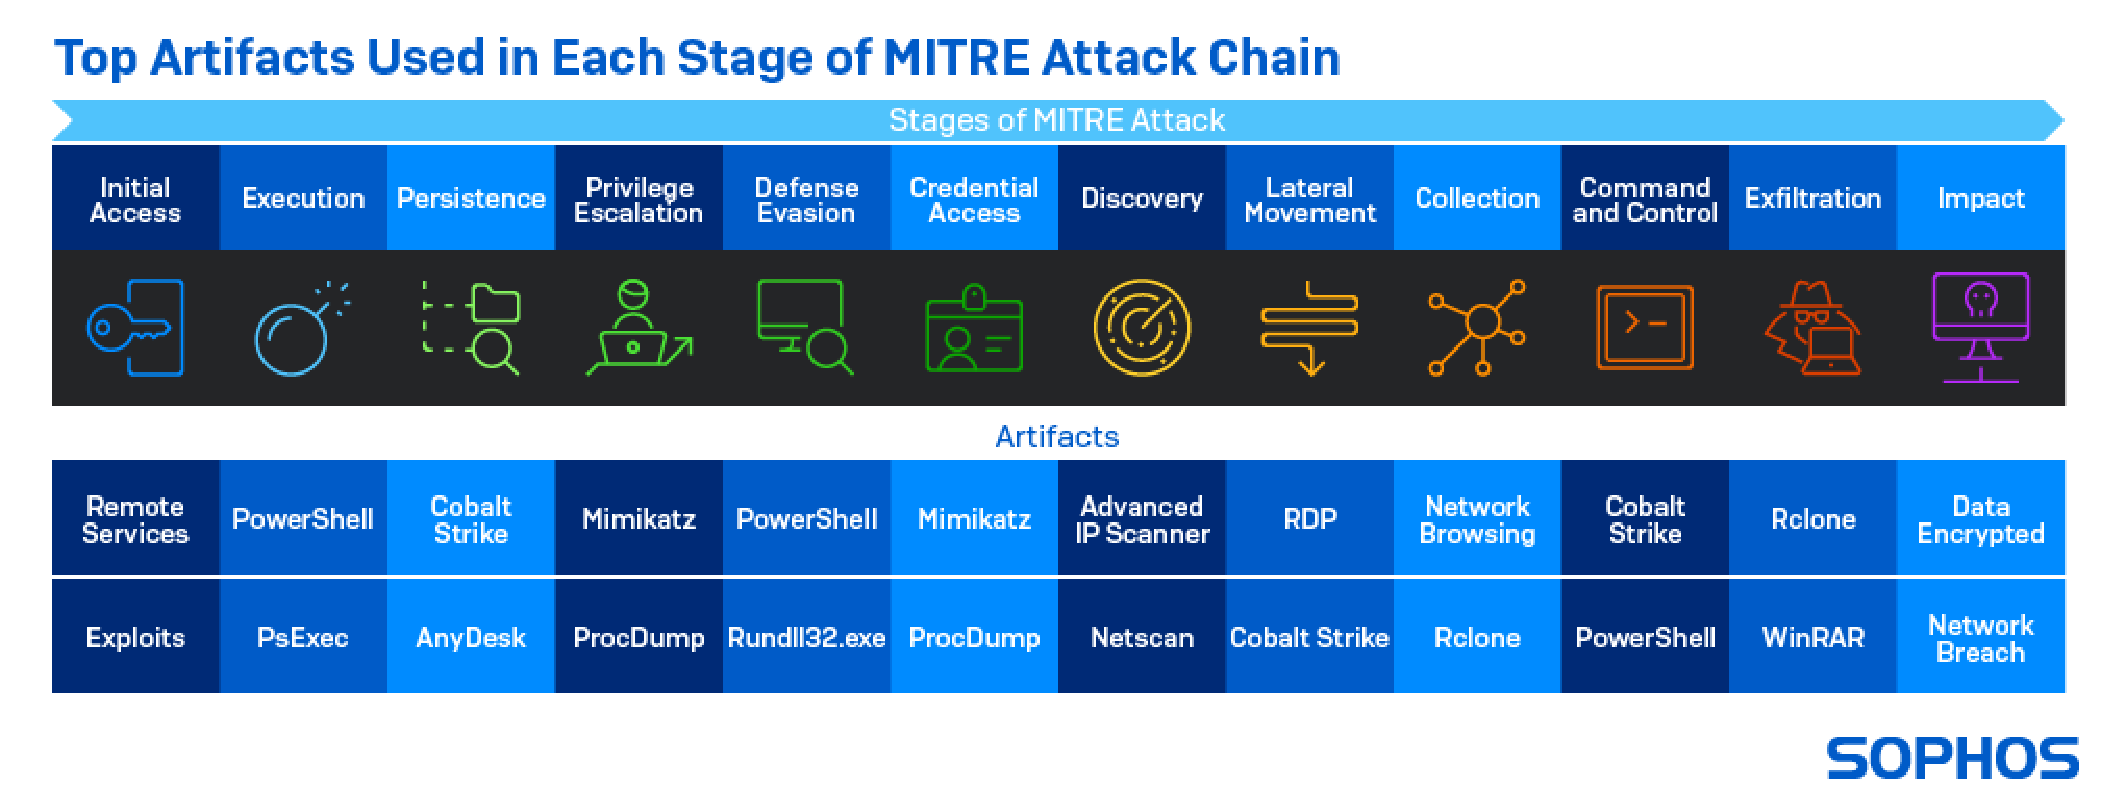
\includegraphics[width=0.8\columnwidth]{doc/img/mitre-attack-chain.eps}
  \end{center}
  \caption{Overview of each stage in MITRE ATT\&CK framework.
    Some stages such as Reconnaissance are omitted for simplicity. \cite{mitre-explained}}
  \label{fig:mitre-attack-chain}
\end{figure}

本節では,すべてのランサムウェアが通過するステージであるInitial Accessステージに焦点を当て,感染リスクの緩和について述べる.
SpyCloud社 \cite{spycloud-ransomware} によると,ランサムウェアのInitial Accessに利用される手法として2023年に最も多く報告されたものは
フィッシング,サードパーティアプリケーションのIAM設定の不備,cookie窃取によるセッションハイジャックであった.
これらの手法に対する一般的な対策を\tabref{tab:initial-access}に示す.
\begin{table}[t]
  \centering
  \label{tab:initial-access}
  \caption{Techniques for Initial Access and general countermeasures}
  \begin{tabular}{|c|c|}
    \hline
    \textbf{Initial Accessの手法} & \textbf{対策} \\
    \hline
    フィッシング                     &
    \begin{tabular}{c}
      メールフィルタリングを強化する \\
      組織構成員の教育を行う
    \end{tabular}
    \\
    % Email filteringUser awareness training,         \\
    \hline
    IAM設定の不備                   &
    \begin{tabular}{c}
      多要素認証を導入する
      % Email filtering \\ User awareness training
    \end{tabular}
    \\
    \hline
    Cookie窃取によるセッションハイジャック     &
    \begin{tabular}{c}
      Secure属性やHTTPOnly属性を強制する \\
      多要素認証を導入する
    \end{tabular}
    \\
    \hline
  \end{tabular}
\end{table}

\section{ランサムウェア検知}
\subsection{特徴量}
ランサムウェアを検知する手法で用いられる特徴量は,
実行ファイルの解析から得られる静的データと,実行ファイルを実行した際にプロセスの振る舞いから得られる動的データに分類される.
静的データを用いた検知を静的検知,動的データを用いた検知を動的検知と呼ぶ.
静的検知と動的検知は組み合わせて使用されることもあり,これをハイブリッド検知と呼ぶ.

静的検知では実行ファイルにおけるランサムウェア特有の構造的特徴を分析する.
典型的な静的データはファイルのハッシュ値,文字列,関数呼び出しなどである .
文字列としては"ransom"や"bitcoin"などのランサムノートに頻出する文字列や,
過去にランサムウェアが使用していたドメイン文字列やIPアドレスなどが確認される\cite{berrueta2019survey}.
また関数呼び出しについては,暗号化やファイルアクセスといった操作の有無を,ランサムウェアと良性アプリケーションの区別に使用することができる \cite{Evolution-Ransomware}.
しかし,静的データは一般に難読化や圧縮などの手法に弱く,さらに新種のランサムウェアに対して有効ではないことが多いという問題が指摘されている \cite{mitigation-modern}.

動的検知では実行中のプロセスの振る舞いを分析する.
ランサムウェアは特定のディレクトリ以下のファイル一覧を取得して各ファイルを暗号化する挙動を繰り返し行うことから,
ファイルシステム上の操作,暗号化ライブラリやAPIの呼び出しが特徴量として使用されることが多い \cite{Evolution-Ransomware}.
またランサムウェアがファイルに書き込むデータは暗号化されているため,
書き込まれるデータのエントロピーを利用する手法も複数存在する \cite{kharaz2016unveil,kharraz2017redemption}.
ただし書き込みデータのエントロピーはファイル圧縮などの正常アプリケーションにおいても高くなるので,エントロピーはその他の特徴量と組み合わせて使われる傾向がある \cite{berrueta2019survey}.

\subsection{検知レイテンシ}
動的検知あるいはハイブリッド検知において,ランサムウェアが実行されてから検知されるまでの時間を本稿では検知レイテンシと呼ぶ.
検知レイテンシが小さければランサムウェアの被害を抑えることができるため,検知手法の評価指標として重要である.
例えばRATAFIA \cite{alam2019ratafia} はオートエンコーダを用いた検知手法で,WannaCryを含む変種を最大5.3秒で検知した.
また,RWGuard \cite{mehnaz2018rwguard} はデコイファイル,プロセス監視,ファイル監視を組み合わせてレイテンシの削減を目指した手法であり,
評価実験ではランサムウェアのプロセスを9秒未満で特定した.
Brownorら \cite{brownor2024ransomware} は提案した検知手法の検知レイテンシをCPU使用率ごとに測定し,
使用率が90\%の設定でも評価に用いたランサムウェアサンプルを3秒未満で検知することができた.

検知レイテンシはランサムウェア攻撃を迅速に終了させられるかどうかという観点において重要な指標であるが,
検知レイテンシの評価を行っている研究が少ないことが指摘されている\cite{alam2019ratafia}.
例えばいくつかの研究では,提案手法の検知精度を最大化するために,30日間などの非常に長い期間での評価を行っているものがある \cite{mitigation-modern}.

\section{ランサムウェア被害からの復旧}
\subsection{バックアップによる復旧}
\subsection{暗号化鍵の取得による復旧}
\ref{subsec:encrypt-algo}節で述べたように,共通鍵暗号では暗号化と復号に同じ鍵を使用する.
そのため共通鍵暗号を利用するランサムウェアに対しては,暗号化に使用される鍵を取得することができればデータを復号することができる.
PayBreak \cite{kolodenker2017paybreak} はこの点に着目して開発された手法で,Windows OSが提供する暗号化ライブラリを
フックして暗号化鍵を取得する.
取得された鍵は事前にユーザが登録した公開鍵によって暗号化されたのち,追記のみが可能なデータストアに保存される.
\begin{figure}[t]
  \begin{center}
    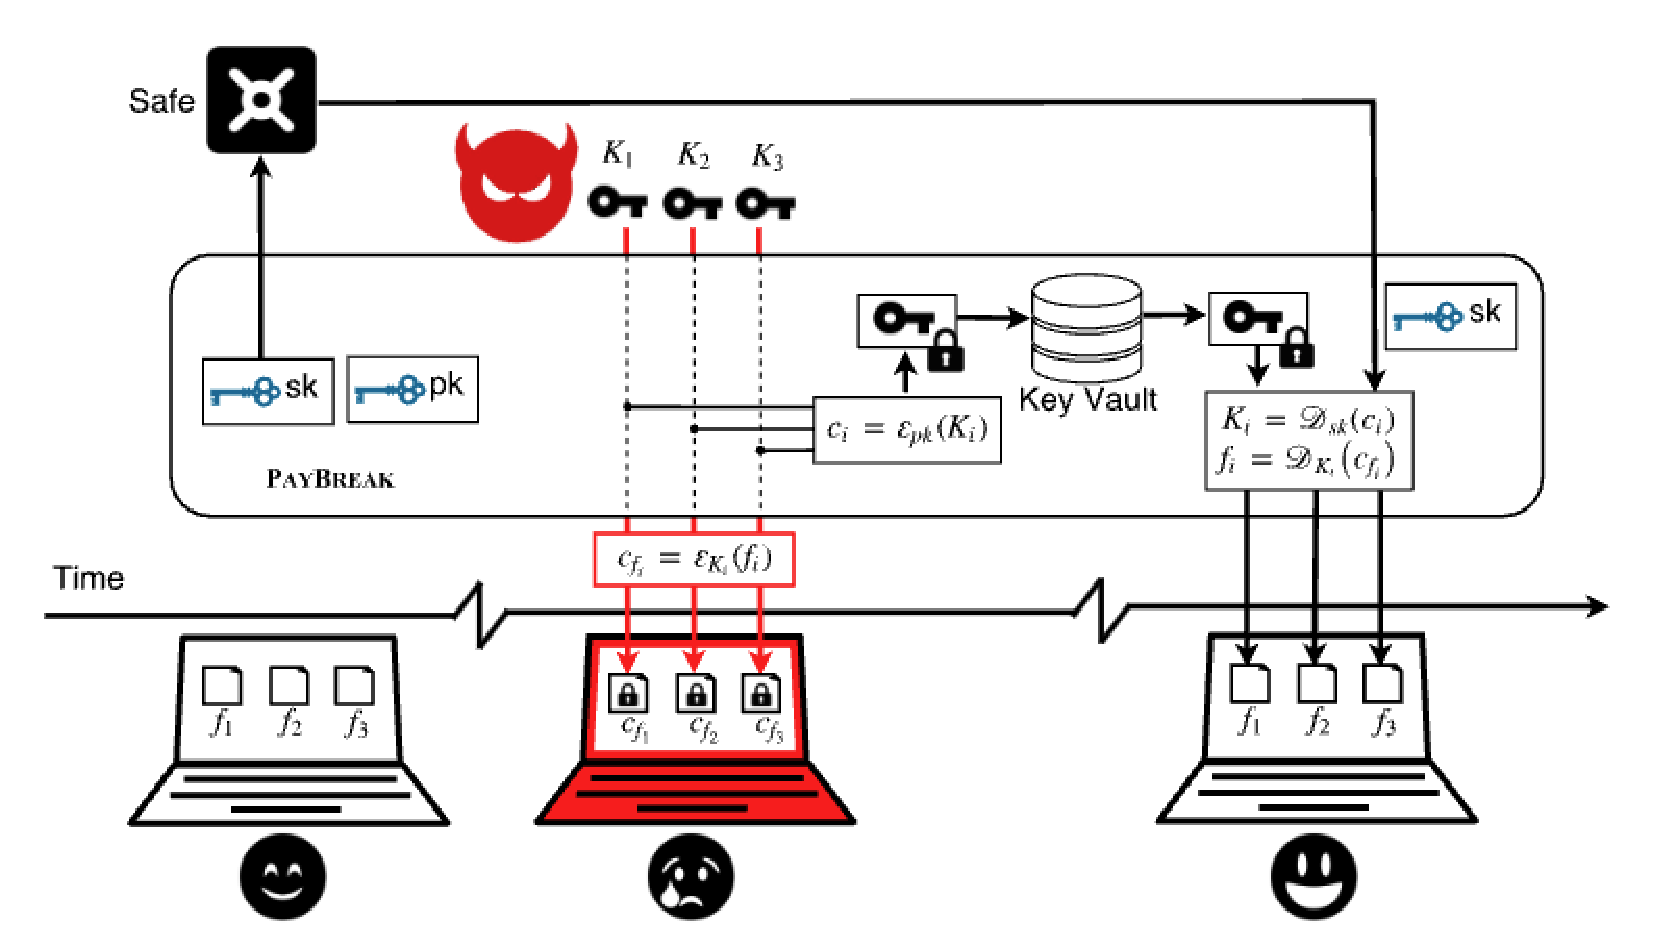
\includegraphics[width=0.8\columnwidth]{doc/img/paybreak-overview.eps}
  \end{center}
  \caption{Overview of PayBreak. \cite{kolodenker2017paybreak}}
  \label{fig:paybreak-overview}
\end{figure}
PayBreakは暗号化ライブラリの動的リンクと静的リンクの両方に対応している.
さらに代替となる暗号化ライブラリが登場した場合でも,マルウェア解析によって一度暗号化関数を特定することができれば,
その関数をフック対象として容易に追加することができる.
しかしながら,PayBreakは非対称鍵暗号を利用するランサムウェアには対応していない.

\subsection{SSDの特性を利用した復旧}
\subsection{ファイルシステムの拡張による復旧}


